\chapter{Results}
\label{ch:results}

The validation of \Cref{ch:validation} established that the renderer is \emph{correct}; this chapter
measures how fast the correct renderer is. All numbers are taken at the renderer's
validated production configuration on the RTX~3090 (\Cref{sec:setup}): the analytic built-in sphere,
multiple-importance-sampled direct lighting, per-asset calibrated caps, exact
\(\operatorname{erf}\). None of the opt-in variants of \Cref{ch:optimization} (product-RIS,
fast \(\operatorname{erf}\), tessellated shell, SER) is enabled. The
reference throughout is Condor's Mitsuba \texttt{volprim} implementation of
DSYG~\cite{DSYG} on the same GPU. Beyond the headline equal-quality result (\Cref{sec:results-perf}),
the chapter reports four axes on which the renderer can be compared to that reference independently
of raw frame time. \Cref{sec:results-firefly} examines the energy bias and firefly behaviour of the
two renderers' direct-lighting estimators. \Cref{sec:results-memory} reports the device-memory footprint
and what per-asset cap calibration saves. \Cref{sec:results-startup} measures the start-up and
iteration latency that matter for an interactive workflow. \Cref{sec:results-generalisation} runs a
cross-renderer agreement check that qualifies further assets for comparison. A final section measures how render time scales with primitive count
(\Cref{sec:results-scaling}).

\section{Equal-quality performance versus Mitsuba}
\label{sec:results-perf}

\textbf{Goal:} the headline question. At equal quality, which of the two renderers' fast
estimators is faster on the environment-lit showcase? This renderer's MIS direct lighting is
measured against the reference's corrected next-event
estimator~\cite{KramarzVolprimFixes2026}. (Arm labels and ``shipped'' as defined in
\Cref{sec:reference-problem}.)

\textbf{Setup:} \Cref{ch:validation} certified that
both systems converge to the same image. The comparison therefore pits the two production
fast paths against each other on equal terms, as the
two production fast paths. Both arms render the showcase ($900\times600$) under the
conventions of \Cref{sec:setup}.

\textbf{Result:} per sample, the corrected reference is the
\emph{less} noisy of the two ($k$-ratio \num{0.785}).\footnote{$k_{\text{nee}}/k_{\text{ours}} = \num{0.785}$, \num{95}\,\% CI $[\num{0.734},
\num{0.842}]$; raw (unclipped) basis \num{0.770}. Conventions: \Cref{sec:setup}. Specific to this
experiment: the $k$-ratio is computed at the \num{64}-spp anchor from \num{16} seeds per
arm, with each arm's clip threshold from its own anchor stack (not from all spp pooled).
CIs are from \num{2000} bootstrap resamples in which each arm's seeds are resampled under
its \emph{own} independent index set---a shared set would spuriously correlate numerator
and denominator and narrow the interval. The speedup CI is the $k$-ratio CI scaled by the
locked-clock median time ratio; the timing spread ($\le$\num{1.2}\,\%) is not propagated.
The flat $1/\mathrm{spp}$ curves of \Cref{fig:likeforlike-equalvar} verify $k$'s
spp-invariance.} Per second, this renderer
is \num{3.47}$\times$ faster: \num{120.4} versus \SI{417.2}{\milli\second} per sample at
\num{256}\,spp. Timing is at locked clocks, arms interleaved, steady-state medians after a
warm-up render, so JIT compilation is excluded on both sides.\footnote{Repeat spreads
$\leq\num{1.2}\,\%$.} The net equal-quality advantage is
$\mathbf{\num{2.72}\times}$ (\num{95}\,\% CI $[\num{2.54},
\num{2.92}]$)~(\Cref{fig:likeforlike-equalvar}). Two fairness notes close the
protocol. Neither estimator produces fireflies here, so the two variance conventions of
\Cref{sec:setup} nearly coincide and the clipping does no work.\footnote{They agree within
\num{5.2}\,\% (ours) and \num{3.2}\,\% (reference); the raw-basis advantage is
\num{2.67}$\times$.} And the reference is timed in
its shipped configuration, shadow-march early-out
enabled, which is its \emph{faster} setting.

\begin{figure}[tb]
  \centering
  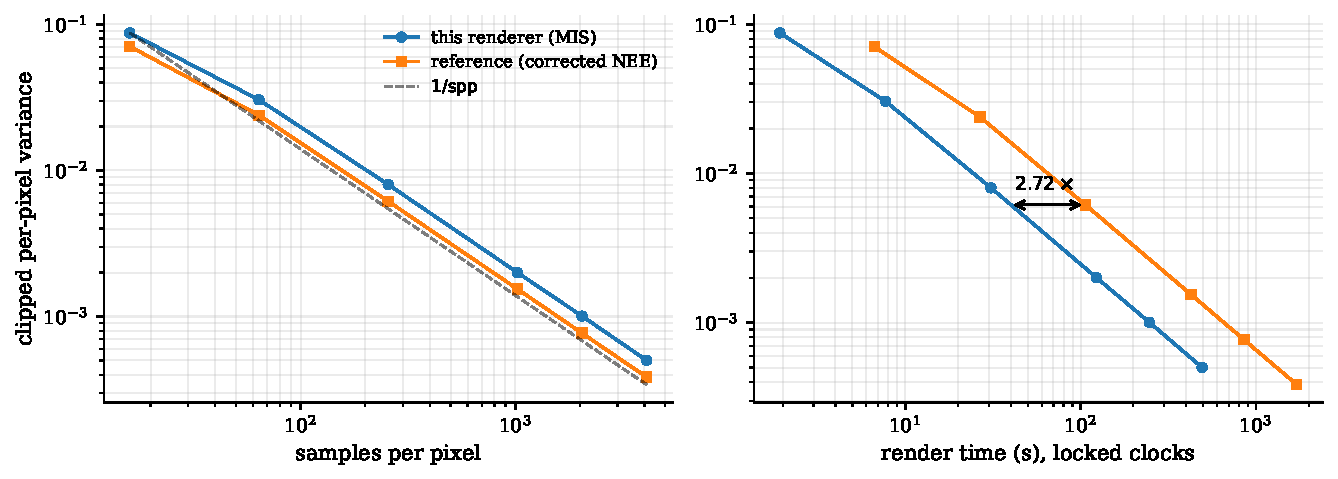
\includegraphics[width=\linewidth]{figures/likeforlike_equalvar.pdf}
  \caption{Equal-quality comparison against the corrected reference: clipped per-pixel variance versus sample count (\emph{left}) and
versus wall-clock render time (\emph{right}) on the cloud--meadow showcase,
\num{16}--\num{4096}\,spp at locked clocks; seeds per point: \num{16} on both arms at the
\num{64}-spp anchor, \num{8}/\num{4} (ours/reference) at \num{256} and \num{1024}, \num{4}
elsewhere. On these log--log axes an unbiased estimator is a straight line of slope $-1$
(variance halves per doubling of spp); residual bias would flatten into a floor. The
horizontal gap on the time panel is the equal-quality advantage: \num{2.72}$\times$ clipped
(raw basis \num{2.67}$\times$). The two panels answer different questions: per sample
(left) the corrected reference is the less noisy arm; per second (right) this renderer
reaches any target variance sooner. Neither arm claims both.}
  \label{fig:likeforlike-equalvar}
\end{figure}

\paragraph{Context: the reference as shipped.} The reference as shipped
(\Cref{sec:reference-problem})---the code as its users obtain it---has no correct fast path on this
medium. Its next-event estimator does not converge to the correct image. In the benchmarked revision
it fails through a gross energy bias; in the current upstream revision it fails through the issues
diagnosed in \Cref{sec:results-firefly}. Its only correctly-converging configuration is
the analog mode, which is firefly-dominated under this illumination (\Cref{sec:results-firefly}); a
comparison against it would measure the shipped code's limitations rather than estimator quality.

\paragraph{Isolating the sampler.} To separate the \emph{sampler} from the direct-lighting estimator,
the two renderers can be compared in the \emph{same} (analog) mode---no NEE on either side. Under the
meadow environment this comparison is metric-unstable, because this renderer's analog variance is
firefly-dominated (rare bright-sun escapes). Raw per-pixel variance favours the reference while
firefly-clipped variance (\Cref{sec:setup}) favours this renderer: the two conventions disagree
on the winner, so no single equal-quality number is meaningful there. A
\emph{flat} (uniform) environment removes the fireflies on both sides and makes the comparison stable.
One convention decides this comparison: the \emph{reconstruction filter}. It is
matched---box on both arms, as everywhere in this
thesis (\Cref{sec:setup}).\footnote{The filter matters because a wide filter averages neighbouring samples, lowering
per-pixel variance by roughly $3\times$. An earlier mismatched-filter reading (the
reference's default Gaussian against this renderer's box; ${\sim}5\times$ apparent gap,
net $0.83\times$) is withdrawn in the measurement record (\texttt{analog\_conv}).} On the matched
basis, the argmin sampler is \num{1.6}$\times$ noisier per sample but renders \num{4.6}$\times$
more samples per second. The \emph{net} equal-quality advantage is $\mathbf{\num{2.87}\times}$.\footnote{Variance
ratio \num{1.59}, constant across a \numrange{16}{512}\,spp sweep, \num{8} seeds per budget; one \num{512}-spp reference seed was discarded during the same logged contention episode
(the measurement record keeps the log), and the contended timing runs were excluded
likewise. Both
estimators are unbiased, with converged means agreeing to
\num{0.02}\,\%. The time ratio, and with it the net figure, is power-dependent and rises at lower
power caps.} The per-sample gap has a known cause: the smooth-weight-versus-coin-flip
estimator trade-off dissected
in the negative results of \Cref{sec:autopsies}. The architectural contribution
(\Cref{ch:architecture}) is therefore a \emph{structural, throughput} simplification: it
removes the march, the sort, and the root-find. Its
per-sample speed more than carries its per-sample variance cost, even with no direct-lighting
estimator in the loop. Under the peaky illumination of production scenes, the MIS estimator then
adds the variance half (\Cref{sec:ris}).

\Cref{tab:likeforlike} summarises the three comparisons side by side.

\begin{table}[htp]
  \centering
  \small
  \begin{tabular}{@{}lllr@{}}
    \toprule
    comparison & env.\ & isolates & equal quality \\
    \midrule
    ours (MIS) vs.\ reference (corrected NEE) & meadow & fast paths & $\mathbf{2.72\times}$ \\
    ours (analog) vs.\ reference (analog) & flat & sampler alone & $\mathbf{2.87\times}$ \\
    \bottomrule
  \end{tabular}
  \caption{The two equal-quality comparisons, each isolating a different question: the production
fast paths under the meadow (against the corrected next-event
reference~\cite{KramarzVolprimFixes2026}), and the flat-field analog--analog matchup
isolating the sampler ($1.6\times$ noisier per sample, $4.6\times$ faster, matched box
filters). Comparisons against the shipped code's analog mode are not tabulated
(\Cref{sec:results-firefly} characterises that configuration's variance).}
  \label{tab:likeforlike}
\end{table}

\paragraph{The advantage is environment importance sampling.} On a flat environment the MIS
estimator carries no advantage at
all: its per-vertex next-event estimation is wasted work when every direction returns the same
radiance. The headline margin is thus the
product of
two separable factors. The sampler's throughput advantage is environment-independent: it
carries the flat analog--analog matchup on its own. The MIS estimator's variance advantage
is specific to peaky illumination---the payoff of importance-sampling a bright, concentrated
HDR environment. This mirrors the resampled direct-lighting result of \Cref{sec:ris}, where the same
environment-sampling estimator helps under peaky illumination and is counterproductive on
flat. The estimator half of the renderer's advantage is therefore largest for the peaky
HDR environments typical of production lighting.

\paragraph{Beyond the cloud.} The bunny~\cite{TurkLevoy1994} (\num{25600} Gaussians) renders in \SI{50.4}{\second} at
\num{64}\,spp, \(512\times512\), under the meadow environment (the white-constant scattering configuration of
\Cref{tab:asset-cost} is \SI{53.9}{\second}; same order), with zero cap overflows. It is the densest
asset exercised. Via its one Gaussian-kernel fit (the asset's other fits use Gabor kernels, which this
renderer cannot consume; \Cref{sec:limitations}), it is also parity-checked against Mitsuba in \Cref{sec:results-generalisation} (converged-mean
ratio \num{0.9984}). Its memory is reported in \Cref{tab:vram}.

\section{The reference's fast estimator: diagnosis, correction, certification}
\label{sec:results-firefly}

Beyond speed, the largest cross-renderer difference concerns \emph{correctness under
production settings}. Both renderers have two direct-lighting modes. The \emph{analog} mode is
unbiased but slow: light is gathered only when a path escapes to the environment. The fast mode
estimates direct light explicitly at each scatter vertex. In the reference this is next-event
estimation (NEE), used alone. In this renderer the same shadow-ray idea is one of two combined
direction strategies---environment sampling and phase sampling---weighted by MIS
(\Cref{sec:nee-mis}). On a dense scattering medium the two fast modes
are not interchangeable. \Cref{fig:g1-bias} renders the showcase cloud three ways: this renderer
(certified as ground truth at the noise level by \Cref{ch:validation}), the reference's NEE as
shipped, and the same estimator with this section's corrections applied.

\begin{figure}[htp]
  \centering
  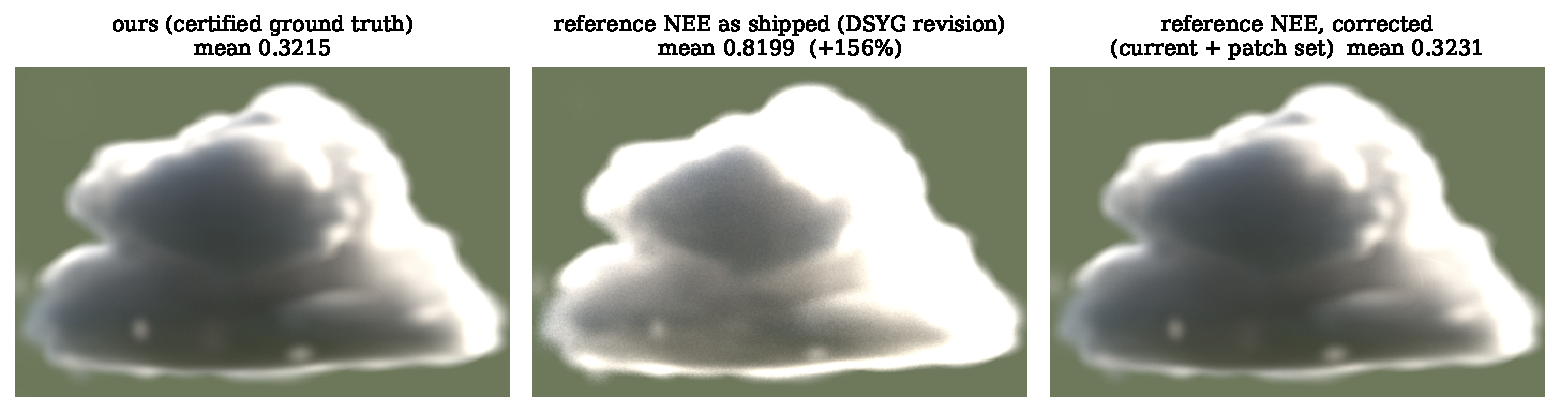
\includegraphics[width=\linewidth]{figures/g1_bias.pdf}
  \caption{Defect and correction: the showcase cloud (meadow environment), identical scene.
  \emph{Left:} ours, certified as ground truth at the noise level by \Cref{ch:validation}
  (spp-weighted mean of \num{18} independent renders, \num{40960}\,spp effective---the
  highest-budget panel of the three; mean \num{0.3215}). \emph{Centre:} the reference's next-event estimator as
  shipped in the benchmarked DSYG revision: mean \num{0.8199}, \num{+156}\,\%. \emph{Right:} the same estimator in the current upstream code
  \emph{with the corrections applied}~\cite{KramarzVolprimFixes2026} (mean of four \num{2048}-spp
  seeds, \num{8192}\,spp effective): mean \num{0.3231}, within \num{0.5}\,\% of the certified ground truth---the like-for-like
  reference of \Cref{sec:results-perf}.}
  \label{fig:g1-bias}
\end{figure}

Anchored to the converged ground truth (mean radiance ${\approx}\num{0.320}$, on which every
unbiased arm of \Cref{ch:validation} agrees to within noise), the shipped reference's
NEE result is \emph{\num{+156}\,\% too bright}. The reference's explicit direct-lighting
estimator does not converge to the correct image on this medium; the analog mode is therefore its only
configuration that does. (The current upstream revision as shipped repairs the over-count but, until the corrections
are applied, under-counts instead: \num{-41}\,\% on a single \num{2048}-spp render.)

The sequence spans several code revisions, so \Cref{tab:revision-timeline} fixes the timeline
once; every other mention in this thesis refers back here. Throughout, the findings concern the
released implementations, not the method they implement; no published DSYG result is
re-evaluated here.

\begin{table}[htp]
  \centering
  \small
  \begin{tabular}{@{}p{6pt}>{\raggedright\arraybackslash}p{\dimexpr\linewidth-236pt-6\tabcolsep\relax}>{\raggedright\arraybackslash}p{125pt}p{105pt}@{}}
    \toprule
    & revision & fast estimator on the showcase & status in this thesis \\
    \midrule
    1 & DSYG release (\texttt{volprim}, \texttt{622fabd}) & $+156\,\%$ over-count (\Cref{fig:g1-bias}) & benchmarked throughout \\
    2 & current upstream rewrite (\texttt{GaborVolumes}) & over-count gone; new issues, $-41\,\%$ & diagnosed here \\
    3 & row 2 $+$ this work's five corrections (PR~\cite{KramarzVolprimFixes2026}) & agrees at the noise level & all ``corrected'' arms \\
    \bottomrule
  \end{tabular}
  \caption{The reference's revision timeline. The released code (row 1) over-counts (cause identified in the text). Its authors' rewrite
(row 2) removed the over-count and carries other issues. With this work's five
  corrections (row 3), the two renderers agree at the Monte-Carlo noise level. The analog
  mode is unbiased in every revision and anchors all cross-checks.}
  \label{tab:revision-timeline}
\end{table}

\paragraph{Where the over-count enters.} Three estimator ingredients recur in this section;
\Cref{sec:nee-mis} defines them formally. \emph{Next-event estimation} pays for direct light
immediately, with a shadow ray toward the light at each scatter vertex. The \emph{analog
continuation} instead lets the path fly on and collects light only if it escapes. A
multiple-importance weight is what keeps two such strategies from counting the same light
twice. The over-count is not an artefact of how the reference was invoked here. It runs at its
documented defaults (Gaussian kernel, bisection solver, path depth \num{128}---deep enough
that truncation can only \emph{darken} the result), and the same over-count appears,
reference-free, in the furnace
test of \Cref{par:furnace}. There, energy conservation alone---no asset, density scale, or
comparison render---forces a correct estimator to return the background.

Its line-level cause was unknown throughout this work's measurements; the bias was
localised, but not to a line. After those measurements, the estimator's author identified
the repaired issue (personal communication, 2026), and his account is verified against
the released source below. The current upstream revision carries a rewritten estimator
that no longer exhibits the over-count (\emph{Upstream follow-up} below).

This thesis therefore claims
only what the measurements localise: the surplus enters at
interior scatter vertices, in the shipped estimator's multiple-importance combination of the
next-event term (analytic shadow-ray transmittance) with the analog continuation. Such a
combination can go wrong in only two ways. The weights may fail to sum to one for some
direction. Or the two
combined terms may integrate \emph{different} media, as when the shadow transmittance and the
flight sampler disagree about the medium's extent or density. Both ways appear in
the later diagnosis of the \emph{current} revision, one instance of each
(\Cref{app:corrections}): a lane-masking issue (a per-sample mask in Mitsuba's vectorised execution) that breaks the weight sum at
depth~\num{0}, and shadow-ray integrals over mass the flight sampler never samples.
For the shipped revision the instance is now identified, and it is of the second kind. In
the released \texttt{eval\_transmittance}, the loop over the primitives overlapping the
scatter vertex reads each one's $\sigma_t$ through a zero-initialised interaction record
whose shape handle is never set; the lookup returns zero, and those primitives drop out of
the shadow transmittance entirely (identified by the estimator's author, personal
communication, 2026; verified in the released source). The shadow ray thus misses exactly
the densest mass at the vertex, so next-event estimation over-counts. Two probes
corroborate the attribution: the release's segment kernel passes the additivity check (the
mirrored-integral class arrived only with the rewrite, \Cref{app:corrections}), and its
full-line shadow march darkens rather than brightens---the $\sigma_t$ zeroing is the
dominant, brightening instance.

This renderer rules out both by construction.
It never MIS-combines next-event estimation against the analog continuation. Instead, it
partitions the \emph{direct} contribution at each vertex between two \emph{light-sampling}
strategies: environment sampling by luminance, and phase sampling. Both strategies carry the
\emph{same} analytic-transmittance measure, so the balance-heuristic partition is exact. The
continuation ray's direct environment term is suppressed, so it is never double-counted against
next-event estimation (\Cref{ch:architecture}). The furnace pass is the evidence that this
partition is exact in practice, together with the converged-mean agreement of the three
arms---this renderer, the analog reference, the corrected-NEE reference---in
\Cref{sec:scattering-ladder} (within \num{0.4}\,\% and
\num{0.5}\,\% respectively).

The measured scaling follows directly from the identified cause: the more primitives
overlap a vertex, the more mass the shadow ray misses. In the furnace of
\Cref{par:furnace} the over-count grows steeply with optical depth even for a \emph{single}
Gaussian. At the Gaussian's centre it rises with density scale: ${\approx}\num{1}\,\%$ at density
scale \num{2}, ${\approx}\num{10}\,\%$ at \num{6}, ${\approx}\num{31}\,\%$ at \num{12}. In the
optically thin limit the analog continuation (the path flown onward) almost always escapes, so
the surplus is small. As
the medium thickens, that escape becomes rare, and the analytic next-event
surplus survives at each interior scatter vertex. \emph{Overlap} compounds this further, and measurably
so. Holding the density scale at \num{6}, the furnace over-count at the medium's centre rises from
${\approx}\num{10}\,\%$ for the single Gaussian (overlap \num{1}) to ${\approx}\num{121}\,\%$ on
the cloud (overlap ${\sim}\num{45}$). That is a roughly twelve-fold amplification from overlap
alone: tens of primitives each contribute the analytic next-event surplus at every interior
vertex. On the cloud at its own density scale \num{7.5} the furnace over-count is already
${\approx}\num{142}\,\%$ at the centre, measured at albedo \num{1} (the furnace setting). The
\num{+156}\,\% of the albedo-\num{0.9} scattering image is therefore the same mechanism; the small
remainder is the surplus being re-scattered by later bounces.

\paragraph{Upstream follow-up.} The over-count above is a property of the reference \emph{revision}
benchmarked throughout this thesis (\texttt{volprim} \texttt{622fabd}). It was subsequently re-tested
against the authors' rewritten integrator (revision \texttt{09be413e}, run on stock Mitsuba~3.8.0),
where the same parameter-free furnace shows the over-count removed ($+9.7\,\%\!\to\!-0.63\,\%$ at
density scale \num{6}). Root-causing first that small residual, and then the rewritten revision's remaining energy
discrepancies (each correction sharpened the next), yielded five
corrections in all (\Cref{app:corrections} reproduces the patch and the per-correction verification):
\begin{enumerate}
  \item \textbf{Depth-0 escape weight.} The camera ray's background contribution cannot be produced
  by next-event estimation, so it must carry unit weight. Instead it was down-weighted by
  $1/(1+(4\pi)^{-2})=\num{0.99371}$, matching the measured furnace deficit to five decimal places.
  The one-line correction restores the furnace to within $-0.004\,\%$, with the analog controls
  exact throughout.
  \item \textbf{Mirrored segment integral.} A sign error in the finite-bounds
  Gaussian line integral evaluated every primitive \emph{mirrored} about the integration segment's
  start---the largest of the five effects, distorting both the sampled medium and the shadow
  transmittance. It stayed hidden for two reasons. In analog mode the sampler is
self-consistent: its decisions and its weights describe the same medium, mirrored or not,
and energy conservation only requires that they agree---so analog furnaces pass at any
density. A single Gaussian, meanwhile, is symmetric, so the mirror maps it onto itself. That is consistent with the sign error
  surviving prior validation.
  \item \textbf{Full-line shadow march.} The shadow march integrated each primitive over its
  full infinite line rather than over the remaining segment. The
  spaced-chain furnace of \Cref{app:corrections} (a line of identical Gaussians separated by
  gaps; ground truth still exactly $1$) demonstrates this asset-free: shipped deviations
  up to $+4.2\,\%$, ${\le}0.02$ percentage points after the corrections.
  \item \textbf{Support-tail mass.} Next-event transmittance counted Gaussian tail mass outside the
  support ellipsoid that the flight sampler truncates (verified in \Cref{app:corrections}).
  \item \textbf{Phantom re-entry.} Found last, on the real asset only. The traversal loop
  double-counted a primitive's optical depth whenever the fixed respawn epsilon undershot the
  single-precision entry point of a small anisotropic primitive. It was isolated in absorption mode---deterministic, no scattering---on an extract of the
cloud's dense core (\num{85} primitives, few enough that every chord's closed-form optical
depth can be summed exactly in float64) and checked against that prediction.
\end{enumerate}
The complete correction is five fixes of $+30/-6$ diff lines in two files.\footnote{A companion commit applies the same mirrored-window correction (fix~2;
\Cref{app:corrections}) to the production mixture kernel, $+2/-2$.} It is
submitted upstream as a pull request~\cite{KramarzVolprimFixes2026} (pending review at the time of
writing). With the corrections applied, the two
renderers agree at the Monte-Carlo noise level everywhere measured. Spaced-chain furnaces agree within
$\pm\num{0.02}$ percentage points across primitive count, spacing, density, solver, and backend. On
the showcase cloud, pixel-level block agreement is \num{0.67}\,\% (meadow) and \num{0.07}\,\%
(uniform environment). The only remaining structure is attributable to the reference's own documented
shadow-march early-out (\Cref{fig:agreement-panels}). One unrelated numerical residue remains
open, far above production densities. The reference's single-Gaussian analog furnace is exact
up to density scale \num{300} but drifts below $1$
beyond ${\sim}10^{3}$.\footnote{\num{0.91}/\num{0.83}/\num{0.64} at
$10^{3}/3{\times}10^{3}/10^{4}$.} The drift is float32
$\operatorname{erf}/\operatorname{erf}^{-1}$ saturation, compounded by expected truncation
at the \num{256}-bounce path cap (a correct walk at these opacities is longer). Against the corrected estimator itself, this renderer remains
\num{2.7}$\times$ faster at equal quality (\Cref{tab:likeforlike}). Since the shipped upstream code
predates these corrections, the analog mode remains the only unmodified reference configuration that
converges to the correct image on the showcase.

Under the meadow illumination the analog mode is
firefly-dominated: the sun's energy arrives only through rare scattering paths that happen to exit
through the small bright disc. Its raw per-pixel variance therefore exceeds its firefly-clipped variance (\Cref{sec:setup}) by a
factor of \num{30}--\num{35}, and over a thousand pixels per \num{64}-spp frame exceed twenty times
the mean. (\Cref{fig:showcase} shows the phenomenon within this renderer's own analog mode.) This is not a
handicap imposed on the reference: its faster estimator, as shipped, is biased here
(\Cref{fig:g1-bias}, centre).

\section{Memory footprint}
\label{sec:results-memory}

\textbf{Goal:} compare peak device memory against the reference, and quantify the effect
of per-asset cap calibration. The renderer's device-memory footprint is dominated not by scene geometry but by the per-ray state
reserved for the path-tracing kernel. The hit buffer and active set (\Cref{sec:gpu-impl}) live in
thread-local memory, which the driver reserves for the GPU's maximum resident thread count. Their
compile-time capacities therefore set a scene-independent floor on device memory. The
acceleration structure itself is comparatively negligible: the instanced unit-sphere GAS is
\SI{0.10}{\mega\byte} compacted for the cloud and \SI{3.97}{\mega\byte} for the \num{25600}-Gaussian
bunny.

\textbf{Setup:} peak device memory per asset, measured the same way for both renderers
(method in \Cref{tab:vram}).

\textbf{Result:} on the cloud, the renderer's peak device
memory is \textbf{\SI{578}{MiB}---\num{31}\,\% below Mitsuba's \SI{838}{MiB}} on the identical scene.
Across the suite the outcome varies. The calibrated build sits below Mitsuba
on the cloud and explosion (\num{31}\,\% and \num{26}\,\% less). It sits above it on the denser tornado
and bunny (\SI{818}{MiB} vs \SI{806}{MiB}, and \SI{900}{MiB} vs \SI{806}{MiB}), whose heavy overlap and
\num{25600} primitives force the largest per-ray hit-buffer reservations. The memory win is therefore real
where the worst-case per-ray hit count is modest and turns into a small overhead on the densest assets---a
direct consequence of the per-ray-reservation model (\Cref{sec:gpu-impl}), not of scene geometry. (The reference figures are for the shipped configuration of the benchmarked revision. The
corrected arms run on the newer upstream codebase, whose baseline footprint is larger for reasons unrelated to the corrections (a newer
Mitsuba/Dr.Jit generation), so it is not tabulated here.)
\Cref{tab:vram} reports the per-asset calibrated peak and, for context, the calibration's saving over a
conservative \(512/512\) fallback (the smallest cap that is guaranteed not to overflow without per-asset
measurement). That saving is the difference between sitting below the reference on memory and above it.

\begin{table}[htp]
  \centering
  \begin{tabular}{@{}lrrrrr@{}}
    \toprule
    Asset & caps (act/hit) & ours & Mitsuba & safe \(512\) & saved \\
    \midrule
    cloud     & 64/96   & 578 & 838 & 1200 & 622 (52\,\%) \\
    tornado   & 112/384 & 818 & 806 & 1200 & 382 (32\,\%) \\
    explosion & 32/160  & 600 & 806 & 1200 & 600 (50\,\%) \\
    bunny     & 80/528  & 900 & 806 & 1200 & 300 (25\,\%) \\
    \bottomrule
  \end{tabular}
  \caption{Peak device memory, all values in MiB (\(\text{saved}=\text{safe}-\text{ours}\);
caps act/hit ${=}$ \texttt{MAX\_ACTIVE\_PRIMS}/\texttt{HIT\_BUFFER\_CAPACITY},
\Cref{sec:gpu-impl}). Mitsuba is
  measured on all four assets under each asset's matched config (the bunny via its one
Gaussian-kernel fit,
  which \Cref{sec:results-generalisation} also parity-checks against the reference). Both columns
  are per-process peaks of the same \texttt{nvidia-smi} compute-apps query, polled every
  \SI{150}{\milli\second} during a render. Ours is selected by process id; Mitsuba, launched
  through a wrapper that hides its process id, is instead read as the largest compute-app
  value on the otherwise-idle GPU---its own process, the only compute app present (so the
  columns measure the same quantity). The safe build reserves a flat 1200\,MiB regardless of asset; the calibrated-vs-safe delta
at fixed geometry isolates the per-ray reservation as the dominant term. Per-asset
calibration saves $0.30$--$0.62\,$GiB ($25$--$52\,\%$), tracking the hit-buffer cap (the
near-\(512\) bunny saves least).}
  \label{tab:vram}
\end{table}

\section{Startup and iteration latency}
\label{sec:results-startup}

\textbf{Goal:} for an interactive or iterative workflow the relevant cost is not only the converged
frame time but the fixed latency before the first pixel.

\textbf{Setup:} each timing is the
time-to-first-render on the cloud scene ($256\times256$, \num{16}\,spp), the median of three fresh
processes, isolated as the first render's time minus the steady-state frame time (the settled
per-frame cost after warm-up, \Cref{sec:setup}). \emph{Cold} means an emptied
kernel cache (the true first-session cost); \emph{warm} means the compilation cache is already
populated---the state of every run after the first.

\textbf{Result:} the
reference, built on Mitsuba's just-in-time-compiled Dr.Jit
backend, pays a one-time kernel-compilation cost on each fresh process: \SI{0.78}{\second} warm (cached
kernels) and \SI{2.20}{\second} cold. (The reference's warm and cold figures were each captured once; ours are medians of three.) This renderer's ahead-of-time-compiled OptiX-IR pipeline loads
and launches in \SI{0.39}{\second} (range \SIrange{0.39}{0.45}{\second} across the three
processes)---roughly half the reference's warm start and about a fifth of its
cold start. The advantage is structural---compilation happens at build time---and
independent of the asset, since it is pipeline setup rather than scene work. It compounds
across the many short renders a parameter sweep or a debugging session entails.

\section{Cross-renderer generalisation}
\label{sec:results-generalisation}

\textbf{Goal:} confirm that the correctness is not cloud-specific. The renderer is checked against
the reference on three further DSYG assets---a tornado,
an explosion plume, and the bunny. Condor's native primitive files are used, so both renderers consume identical
geometry (the bunny via its one Gaussian-kernel fit; its Gabor-kernel fits are
unsupported here).

\textbf{Setup:} each is rendered in uniform-albedo-\num{0.9} scattering under a constant-white environment from a matched diagonal
view (the configuration that makes the comparison reference-adjudicable, \Cref{sec:money-shot}).
Renders are at
$512\times512$ and $\sigma_t$ scale \num{10}, each arm a single \num{256}-spp render. The
metric is the image-mean radiance ratio. A ratio of \num{1} means the two renderers put the
same total light into the image.

\textbf{Result:} against Mitsuba-analog all three assets agree with the reference to within
\num{0.16}\,\%---the cloud's level (tornado \num{0.9991}, explosion \num{1.0001}, bunny
\num{0.9984}; four digits, as the single-seed image means support). The bunny's \num{0.16}\,\%
is the largest, consistent with the overlap residual of \Cref{ch:validation}: that residual
appears where primitives overlap most, and the bunny is the most heavily overlapped asset. \Cref{fig:generalisation} then repeats the three-asset check in this thesis's
strongest configuration. The same assets and camera are rendered under the \emph{peaky meadow} illumination of the
showcase, against the reference's \emph{corrected} next-event
estimator~\cite{KramarzVolprimFixes2026} (per asset: ours \num{16}$\times$\num{256}\,spp, reference
\num{4}$\times$\num{1024}\,spp---the same \num{4096}-spp effective budget on both arms). This is the regime in which an environment-orientation, shadowing,
or direct-lighting error would be glaring. The mean ratios are \num{0.9952} (tornado), \num{0.9988} (explosion), and \num{0.9958}
(bunny): the same ${\sim}0.5\,\%$-scale offset the cloud-level certification resolves
(\Cref{ch:validation}). The difference image is uncorrelated pixel noise plus that
known core-level offset, with no spatially coherent pattern beyond it. A real discrepancy
would leave a coherent pattern (\Cref{sec:reference-problem}); none is present. This bounds
any systematic difference below the precision the test resolves, rather than proving it
exactly zero. These
gates confirm that the renderer's correctness is not cloud-specific but holds across three assets spanning
sparse (tornado) to dense, heavily-overlapped (bunny) media, under both uniform and sharply directional
lighting.

\begin{figure}[htp]
  \centering
  
\includegraphics[width=\linewidth]{figures/generalisation.pdf}
  \caption{Cross-renderer generalisation on three further DSYG assets, uniform-albedo-\num{0.9}
  scattering under the peaky meadow environment from a matched diagonal view; panels are cropped to the
  asset. \emph{Left to right:} ours (average of \num{16} \num{256}-spp seeds), the reference's corrected
  next-event estimator~\cite{KramarzVolprimFixes2026} (average of \num{4} \num{1024}-spp seeds), and the
signed relative difference ($\pm\num{5}\,\%$ full scale; conventions, \Cref{sec:setup}).
  The mean ratios are \num{0.9952} (tornado, top), \num{0.9988} (explosion, middle), and
\num{0.9958} (bunny, bottom), and the difference is speckle plus the core-level ${\sim}0.5\,\%$ offset,
with no structure beyond it: the agreement is neither cloud-specific nor
uniform-lighting-specific.  (A separate constant-white run of the same
  matched-camera pair, against the corrected next-event arm, agrees to
  \num{0.9991}/\num{0.9999}/\num{0.9981}; the gate in the body is against Mitsuba-analog.)}
  \label{fig:generalisation}
\end{figure}

\section{Scaling with primitive count}
\label{sec:results-scaling}

\textbf{Goal:} determine how render time depends on the primitive count $N$. The
architecture's claim (\Cref{ch:architecture}) is that per-ray cost is set by the
primitives the ray crosses rather than by the scene total. The claim has a testable
consequence: if the number of primitives each camera ray crosses is pinned \emph{by
construction}, render time should track the crossing count no matter how large $N$
becomes.

\textbf{Setup:} three synthetic families, each holding the rendered content and its total
optical depth fixed while only $N$ changes. The \emph{sheet} is an $n\times n$ lattice in
a fixed footprint, kernels shrunk with the spacing so that every ray crosses at most four primitives at any $N$. The \emph{cube} is an $N{=}n^3$ lattice: an axis-aligned ray crosses its $n$ layers. The \emph{stack} lines $N$ frame-covering
Gaussians up along the view axis: every ray crosses all $N$. The three families pin the
crossing count to the three laws a lattice can realise: constant, $N^{1/3}$, and $N$. The two extremes bracket every possible asset---the sheet is the case where
added primitives should cost nothing, the stack the case where each one is paid in
full---and the cube most closely models real volumetric structure, a blob a ray passes
partway through. The renderer's built-in hit counters (the cap-measurement mode of \Cref{sec:gpu-impl})
confirm the constructed crossing counts at every one of the \num{52} sizes: at most
\num{4} hits per ray on the sheet at all $N$ (a ray near a lattice-cell corner lies inside the four neighbouring primitives; kernel
size is tied to the lattice spacing, so this worst case is the same at every $N$), exactly $4n$ on the cube (an axis-aligned ray meets all $n$ layers at the same lateral
offset, so the per-layer worst case of four repeats in every layer), and exactly $N$ on the
stack. All families render in absorption against a constant white environment
(deterministic, \Cref{sec:setup}) from the same camera at $512\times512$ and
\num{64}\,spp, under one fixed binary---the fixed-cap safe-\num{512} build of
\Cref{sec:results-memory}---so the per-ray buffer reservation, which itself affects
kernel occupancy, is identical across the sweep and only the scene varies. Timings
follow the protocol of \Cref{sec:setup} (median repeat spread \num{1.4}\,\%).

\textbf{Result:} render time follows what a ray crosses rather than the scene total
(\Cref{fig:scaling}). The stack, where every ray crosses all $N$, follows slope \num{1} on the log--log axes
(fitted \num{1.01} over its upper half): each crossed primitive adds about \SI{5.5}{\milli\second} of frame time---the full
per-primitive \emph{transport} work: chord intersection, optical-depth evaluation, and
scatter sampling. The sheet, where crossings
stay constant, is flat to within $\pm2\,\%$ from $N{=}16$ to $N{=}256$: a $16\times$
increase in primitives at no cost, which is the architecture's claim working as designed.
Past $N\approx256$ the sheet nevertheless turns linear. The rise is not transport---the
rays still cross only four primitives---but the bounce-\num{0} containment scan
(\Cref{sec:wins}): each camera sample checks all $N$ primitives once for those containing
the ray origin, so even primitives no ray ever crosses cost a little per frame. That cost is roughly $20\times$ smaller per primitive than the stack's. Varying one
factor at a time at the largest sheet size\footnote{$N{=}8281$; the sweeps are in the
measurement record.} confirms the attribution: the extra cost grows linearly with the
sample count and with the ray count, while crossings stay at four throughout.
The cube lies between the two regimes, consistent with its $N^{1/3}$ crossing count,
though no pure $N^{1/3}$ stretch is visible: past $N\approx300$ the scan term dominates
its growth as well, and only the joint model resolves its transport share. These mechanisms compose into a cost model,
\[
  t(N) \;=\; t_{0,f} \;+\; a\,N \;+\; b_f\,\#_{\text{crossings}}(N),
\]
with $f$ indexing the family: a per-family constant $t_{0,f}$ (fixed overhead), the scan
term $a N$ with one coefficient $a$ shared by all three families (the loop is the same
whatever the scene), and a transport term $b_f$ per crossing, against the family's
constructed crossing count $\#_{\text{crossings}}(N)$. Fitted jointly to all \num{52} points, the model is approximate rather than exact: for
half the configurations its predicted frame time lands within \num{12}\,\% of the
measured one, and the largest misses (up to ${\sim}30\,\%$) sit at the crossovers where
neither term dominates. The misfit is the model's, not the data's: repeat spreads are
${\sim}\num{1.4}\,\%$.\footnote{At this budget, $a\approx\SI{0.26}{\milli\second}$ per
primitive and the stack's $b\approx\SI{5.5}{\milli\second}$ per crossed primitive---the
${\sim}20\times$ ratio above. The sheet, where transport is constant, pins $a$; the
stack's linear term then measures $b$.}

\begin{figure}[htp]
  \centering
  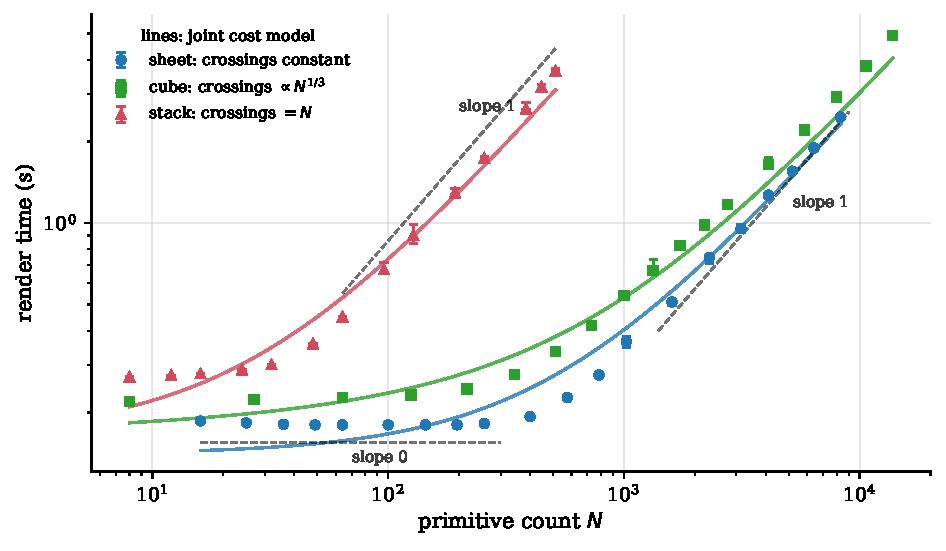
\includegraphics[width=\linewidth]{figures/scaling_v2.pdf}
  \caption{Render time versus primitive count $N$ for three synthetic families whose
per-ray crossing counts are fixed by construction: a constant-crossings sheet, an
$N^{1/3}$-layers cube, and an all-$N$ depth stack. The stack's slope-$1$ behaviour is
per-crossing transport; the sheet's late linear rise is the ${\sim}20\times$ cheaper
bounce-\num{0} containment scan. Solid lines: the joint cost model (per-family constant
and transport term, shared per-primitive scan term); dashed guides mark slopes \num{0} and \num{1}; the two slope-\num{1} guides are
parallel, and the vertical gap between them is the ${\sim}20\times$ per-primitive cost
gap between transport and scan. Log--log; \num{52} configurations, all shown; absorption, one fixed binary,
locked clocks; error bars span the five retained repeats and are mostly smaller than the
markers.}
  \label{fig:scaling}
\end{figure}

The dominant cost follows what rays cross, matching the design goal of
\Cref{ch:architecture}. The subdominant per-sample $O(N)$ scan is a real, quantified
overhead: the fitted coefficient puts it at ${\sim}5\,\%$ of the frame on the
\num{652}-primitive cloud and ${\sim}12\,\%$ on the \num{25600}-primitive bunny, a share
independent of the sample budget since scan and frame scale together. That makes it the
clearest remaining optimisation target. Neither fix was attempted here, but both are
simple: at bounce \num{0} the query point is the camera position, shared by every
sample, so the containing set could be precomputed once per frame; a point query against
the acceleration structure would handle arbitrary origins (\Cref{sec:future-work}).
\Cref{tab:asset-cost} lists the four production assets' operating costs under a matched
configuration; they are not a scaling series, since across real assets $N$ is confounded
with packing density and extent (\Cref{tab:overlap}). Device memory is unaffected
throughout: at fixed caps it is independent of $N$ (\Cref{sec:results-memory}).

\begin{table}[htp]
  \centering
  \begin{tabular}{@{}lrrr@{}}
    \toprule
    Asset & Primitives & Render time & Peak VRAM \\
    \midrule
    cloud     & \num{652}   & \SI{3.65}{\second}  & \SI{578}{MiB} \\
    tornado   & \num{768}   & \SI{5.02}{\second}  & \SI{818}{MiB} \\
    explosion & \num{1024}  & \SI{5.56}{\second}  & \SI{600}{MiB} \\
    bunny     & \num{25600} & \SI{53.9}{\second}  & \SI{900}{MiB} \\
    \bottomrule
  \end{tabular}
  \caption{Production-asset costs under a matched configuration (scattering, albedo \num{0.9},
  white-constant environment, \(\sigma_t\) scale \num{10}, \(512\times512\), \num{64}\,spp, median of three
seeds; peak VRAM from \Cref{tab:vram}). Per-point spreads were not retained, but every
cross-asset difference exceeds the ${\le}\num{1.2}\,\%$ locked-clock timing jitter of
\Cref{sec:results-perf} by an order of magnitude or more. These are operating costs; they
do not form a scaling series, because the assets differ in packing density and extent as
well as count (\Cref{tab:overlap}). The controlled \(N\)-scaling is \Cref{fig:scaling}.}
  \label{tab:asset-cost}
\end{table}


